\documentclass[9pt,twocolumn,twoside]{../../styles/osajnl}
\usepackage{fancyvrb}
\usepackage{listings}
\journal{i524} 

\title{Charge Detection Mass Spectrometry}

\author[1,*]{Scott McClary}

\affil[1]{School of Informatics and Computing, Bloomington, IN 47408, U.S.A.}

\affil[*]{Corresponding authors: scmcclar@indiana.edu}

\dates{project-001, \today}

\ociscodes{Chemistry, Cloud, Hadoop Streaming, HPC, I524, Parallel Computing}
\doi{\url{https://github.com/cloudmesh/sp17-i524/blob/master/project/S17-IO-3011/report/report.pdf}}

\begin{abstract}
A Charge Detection Mass Spectrometry research application is used to
show the benefits of using Cloudmesh and Ansible Galaxy to deploy
software on one or more Virutal Machines in the Cloud. Previously,
this properitery research application was installed and run by hand on
local servers or Supercomputers which turned out to be cumbersome for
the domain scientists. Furthermore, transfering the input data to
remote systems as well as aggregating and visualizing the results is
difficult and tedious. Improving this research workflow by automating
the deployment of the necessary software subsystems in the Cloud
assists in building an efficient, reproducible and scalable Charge
Detection Mass Spectrometry research workflow.
\newline
\end{abstract}

\setboolean{displaycopyright}{true}

\begin{document}

\maketitle

\begin{figure}
\centering
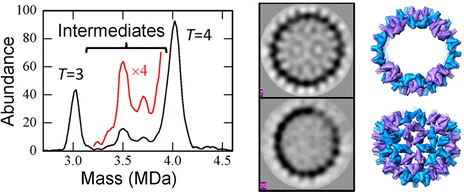
\includegraphics[height=1.35in, width=3.3in]{images/hbvassembly}
\caption{The chart to the left displays an accurate measurement of the
  Hepatitis B virus (HBV) created by the research group's Charge
  Detection Mass Spectrometry research application \cite{247}. This
  detailed mass information is used to create the images shown in the
  middle and to the right, which show 2-D and 3-D models of an
  instance of the HBV.}
\label{fig:hbvassembly}
\end{figure}

\section{Introduction} \label{introduction}
\subsection{Research Background} \label{research-background}
The Martin F. Jarrold research group studies Charge Detection Mass
Spectrometry (CDMS). Their general day-to-day workflow consists of
conducting many scientific experiments using a Mass Spectrometer. This
expensive instrument creates raw frequency data throughout each
experiement. They have developed a Fast Fourier based application
written in Fortran to processes this raw frequency data in order to
determine detailed mass information of the substance used in the
aformentioned experiment. The detailed mass information outputted from
the application is then used to solve important research topics such
as the measurement and classification of the the Hepatitis B
virus. The mass information can be straightforwardly plotted to
determine interesting peaks and valleys when comparing the
mass/abundance of ions and can be used to create graphical
representations of the ions, shown in Figure \ref{fig:hbvassembly}.

\subsection{General Problem} \label{problem}
The Martin F. Jarrold research group generates a lot of raw data that
needs to be processed. For instance, a typical day conducting research
will consist of 8 to 10 one hour experiements with each experiement
generating 2 MB of raw frequency data every half second. Therefore, a
single day of experiements can generate up to 144 GB of data. The
research group must be able to process this data in a similar amount
of time as the time required for the data generation or they will
quickly get inundated in piles of raw data. This day-to-day research
workflow typically strains the research groups local compute
resources. And furthermore, the research group makes algorithmic
changes to the CDMS research application from to time to time which
requires a bulk reprocessing of months or even years worth of raw
data. In this case, the limited compute resources available to the
group becomes a significant limitation to their research.

\subsection{General Solution} \label{solution}
The research group is composed of domain scientists who do not
necessarily have backgrounds in Computer Science. Therefore, a
scalable, efficient, and reproducible solution must be generated to
handle their day-to-day research workflow as well as bulk reprocessing
of months or even years worth of raw data. The solution to their
compute limitations consists of leveraging Cloudmesh and Ansible
Galaxy to deploy their research application and the required software
subsystems on one or more Virutal Machines in the Cloud. The ability
to dynamically modify the number of Virutal Machines and even the
number of Clouds will ensure a scalable, efficient, and reproducible
solution that meets their compute needs. Furthermore, the usage of
Ansible Galaxy will ensure a simple solution that these domain
scientists will be able to master while spending the majority of their
time and effort on their actual research problems.

\section{Execution Plan} \label{plan}
The following subsections act as a timeline regarding how I broke the
project up week-by-week in order to complete the entire project by the
desired deadline. The project execution plan is simply a guide and was
followed diligently; however, some items were pushed slightly
forwards or backwards as technological challenges were faced.
\subsection{March 6, 2017 - March 12, 2017}
This week I installed Cloudmesh on my local machine, created my first
Virtual Machine on the Chameleon Cloud and tested Ansible Galaxy on
remote systems such as one or more Chameleon Cloud VM's. I also wrote
the project proposal, which will eventually become the project reoprt.
\subsection{March 13, 2017 - March 19, 2017}
This week I tested the deployment of the Intel Compiler on one or more
Chameleon Cloud VM's using Ansible Galaxy. I did not expect
significant progress to be made during this weeek given that I was out
of town for Spring Break.
\subsection{March 19, 2017 - March 26, 2017}
This week I attempted to configure the Intel Compiler to use the
Indiana University Intel license server. This required connecting to
Indiana University's VPN from the command line.
\subsection{March 27, 2017 - April 2, 2017}
This week I deployed the Charge Detection Mass Spectrometry along with
the required input data on one or more Chameleon Cloud VM's using
Ansible Galaxy.
\subsection{April 3, 2017 - April 9, 2017}
This week I modified the source code of the OpenMP parallel Charge
Detection Mass Spectrometry application to leverage Hadoop Streaming.
\subsection{April 10, 2017 - April 16, 2017}
This week I benchmarked both the deployment and the analysis on at
least one cloud (i.e. Chameleon Cloud). I also created a method to
aggregate the output from one or more VM's and locally visualize the
results.
\subsection{April 17, 2017 - April 23, 2017}
This week I ensured the reproducibility of my source code as well as
wrote and revised the final version of the report.

\section{Ansible Galaxy} \label{licensing}
Ansible Galaxy was leveraged in order to automate the deoployment of
the required software subsystems, user code and data.

\subsection{Software Subsystems} \label{software}
The CDMS application relies on the Math Kernel Library (MKL) to
leverage efficient Fast Fourier Computations. The application also
leverages the OpenMP parallel framework in order to divide the work
amongst available CPU's. Therefore, in order to compile and run the
application, the Intel compiler is required, which provides the MKL
and OpenMP functionality.

\subsection{User Code} \label{code}
The Martin F. Jarrold Group has written a Fast Fourier Based
application written in Fortran in order to conduct their CDMS
research. This application is approximately 15,000 lines of
code. Depending on the input, about 60\% to 70\% of the compute time
is spent within external MKL libraries conducting FFT calculations.

\subsection{Data} \label{data}
The CDMS application inputs a set of raw 2 MB files. In order to
develop and test the efficiency of the deployment, a small and large
dataset was used. The small test dataset (i.e. 200 files) has a total
size of 400 MB and the large dataset (i.e. 4,506 files) has a total
size of 9.012 GB. A typical dataset for the research group is
approximately the size of the large dataset. In a single day, 7 to 10
datasets are created and need to be processed. When an algorithmic
change occurs to the research application, a large batch of archived
data requires reprocessing. In this case, terabytes of data may be
processed. This is why the parallelization and therefore the
scalability of the application is critical to the Martin F. Jarrold
research group. 

\section{CDMS Research Pipeline} \label{cdms}
\begin{figure}
\centering
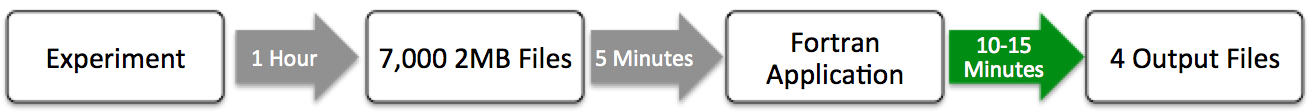
\includegraphics[height=0.45in, width=3.3in]{images/pipeline}
\caption{CDMS Pipeline}
\end{figure}

\section{Licensing} \label{licensing}
\subsection{Deployment and Benchmarking Source Code} \label{source-license}
The source code (i.e. Bash, Ansible, Python) presented is licensed
under the Apache License, Version 2.0 \cite{www-apache-lic}. 
\subsection{CDMS Source Code} \label{cdms-license}
The Martin F. Jarrold Group research group owns all of the rights to
the Fortran Source code and data. All distribution of the application
and data must be consented by the research group.
\subsection{Intel Compiler} \label{intel-license}
The Intel Compiler requires a license in order to complete the
installation. A student license is obtainable for free with an EDU
email address; however, the leveraginng the Indiana University Intel
license server would provide a more complete and reproducible
solution. In order to use the Indiana University Intel license server,
the Virtual Machines be in the Indiana University IP address
space. This can be achieved by connecting each Virtual Machine to
Indiana University's Virtual Private Network (i.e. VPN). In order to
connect to the VPN, one must connect via DUO Authentication (i.e. use
a phone or token to validate). Connecting to IU's VPN from the command
line using Ansible ended up being more of a hassle than it was
worth. 

\section{Benchmark} \label{benchmark}
As discussed in section \ref{code}, the application is parallelized
using OpenMP. Therefore, this application utilizes the avaialable
computational power available. Figure \ref{fig:scalability2} compares
the performance of the application on difference compute resources
(i.e. local servers, Supercomputers and clouds).

The time required to deploy and run the application in the cloud is
shown in the figure \ref{fig:benchmark}. This benchmark includes the
time required for the installation of the software subsystems as well
as the time required to run the application.  \TODO{Add timing
  information for one or more clouds (i.e. Chameleon) to Figure
  \ref{fig:scalability2} and compare the results (if possilbe).}

\subsection{OpenMP Scalability} \label{omp-scalability}
\begin{figure}
\centering
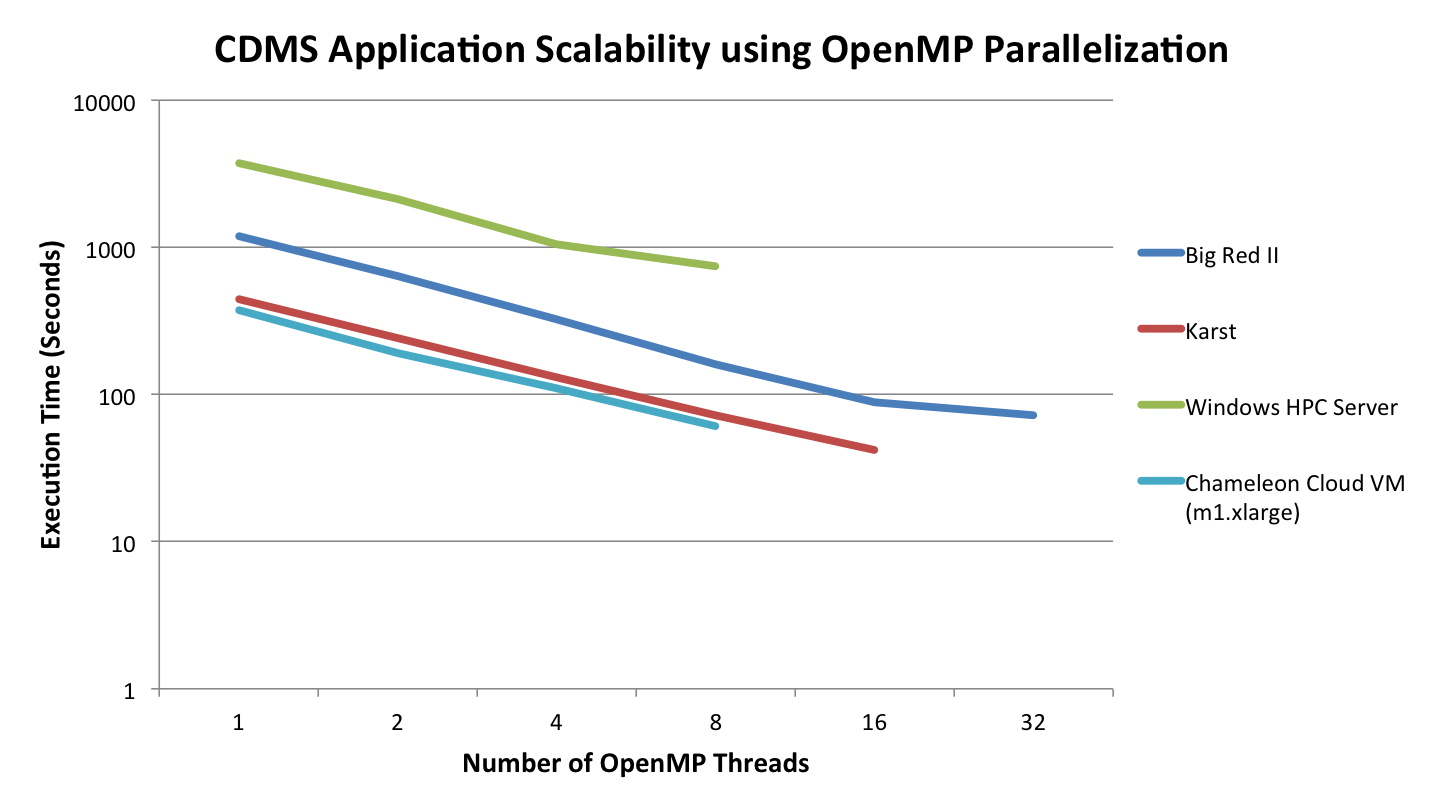
\includegraphics[height=2.3in, width=3.3in]{images/scalability2}
\caption{The figure above shows the scalability (i.e. reduction in
  time-to-solution) as the number of OpenMP threads increase on local
  servers, Supercomputers and Clouds.}
\label{fig:scalability2}
\end{figure}

\subsection{Hadoop Scalability} \label{hadoop-scalability}
The Hadoop Streaming application does not exhibit the desired
scalability. Since the application is essentially a map only Hadoop
application, the performance (i.e. total runtime) of the application
should decrease linearly with an increase in the number of nodes
deployed. However, as the table below indicates, the runtime remains
consistent for all clusters.

\begin{figure}
\centering
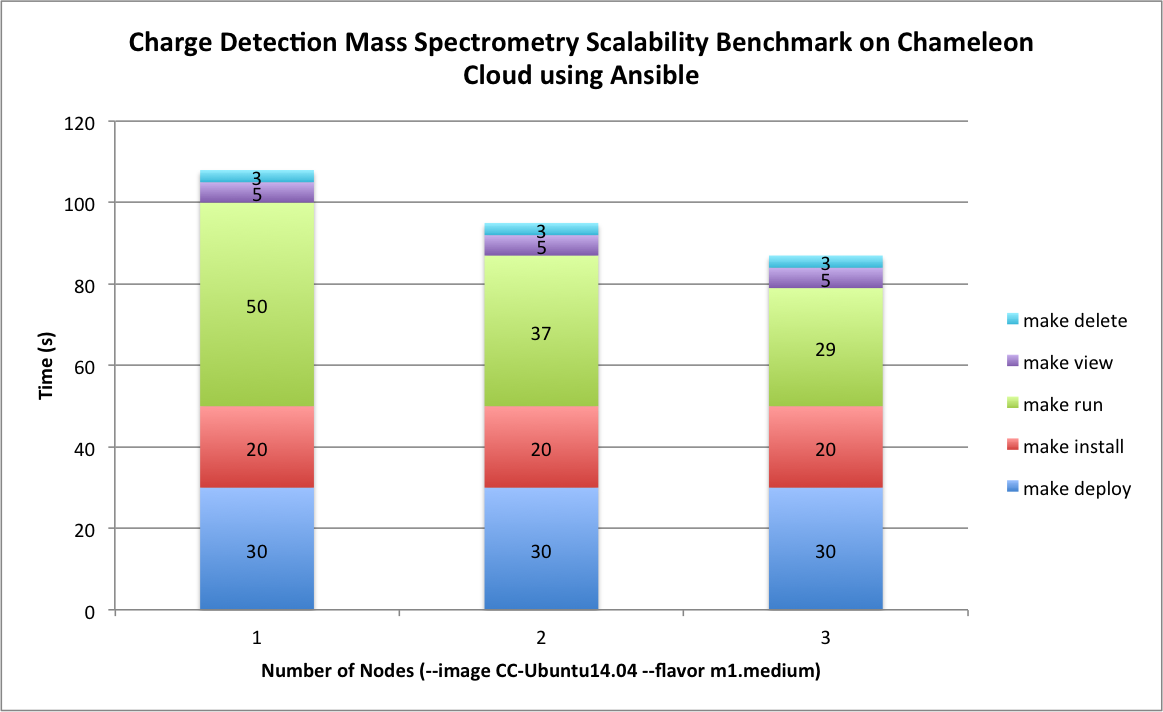
\includegraphics[height=2.1in, width=3.3in]{images/benchmark}
\caption{}
\label{fig:benchmark}
\end{figure}

\section{Reproducibility} \label{reproducibility}
This solution was specifically architected in order to be easily
reproducible. 
\subsection{Requirements} \label{req}
Must have Cloudmesh and Ansible installed locally and must have valid
$\sim$/.cloudmesh/cloudmesh.yaml file stored locally. The cloudmesh
installation is used to launch and manage VM's in the cloud. The
ansible installation is the backbone which initiates the deployment of
the cluster, installation of the required software and benchmarking of
the CDMS application.
\subsection{Fetch Code} \label{git}
The source code is hosted using Github \cite{i524-github}. This
repository contains the required Ansible and Bash scripts used to
automate the research workflow.
\noindent See the following Bash commands:
\begin{lstlisting}[language=bash]
  >> git clone [REPOSITORY]
  >> cd sp17-i524/project/S17-IO-3011/code
\end{lstlisting}
\subsection{Benchmark} \label{benchmark-info}
The benchmark discussed in Section \ref{benchmark} is available for
you to reproduce the results. A single command will deploy the Hadoop
cluster, install required software, run the three versions
(i.e. Serial, OpenMP and Hadoop) of the CDMS application, aggregate
the results, create plots of the output and delete the Hadoop
cluster. Timing information for each stage will be printed to the
screen once the benchmark has completed.
\noindent See the following Bash command:
\begin{lstlisting}[language=bash]
  >> make benchmark
\end{lstlisting}
By default the benchmark will be run on one, two and three
node(s). You can modify the maximum number of nodes (i.e. 5) to be
used in the benchmark with the following command. This will run the
benchmark with one, two, three, four and five node(s).
\noindent See the following Bash command:
\begin{lstlisting}[language=bash]
  >> make benchmark num_nodes=5
\end{lstlisting}
\subsection{Additional Commands} \label{other}
There are many pieces within the benchmark explained in Section
\ref{benchmark-info}. In case you would like to break up the benchmark
into individual pieces, there are seperate Bash commands
available. These commands will deploy the Hadoop cluster, install the
required software subsystems, run the application, view the results
and delete the Hadoop cluster.
\noindent See the following Bash command:
\begin{lstlisting}[language=bash]
  >> make [deploy/install/run/view/delete]
\end{lstlisting}

\section{Conclusion} \label{conclusion}
\subsection{Simplicity} \label{Simplicity}
The use of Ansible Galaxy and Cloudmesh to run the Charge Detection
Mass Spectrometry application in the Cloud (e.g. Chameleon Cloud)
imporved the efficiency, reproduciblity and scalability.
\subsection{Performance} \label{performance}
In comparison torunning on the Indiana University HPC clusters
(e.g. Karst and Big Red II), the application time-to-solution
diminished sigificantly. The most important and useful tool that was
developped as a result of this project was the automation of the
deployment of the necessary software subsystems, the application
itself, the necessary input data and aggregation/visualization of the
output. The use of Ansible Galaxy within this research workflow will
allow the Martin F. Jarrold research group to focus on the details of
their specific research rather than on the details of managing the
software subsystems, running the application and managing the
input/output data.

\section*{Acknowledgements}
The authors would like to thank the School of Informatics and
Computing for providing the Big Data Software and Projects (INFO-I524)
course \cite{www-i524}. This project would not have been possible
without the technical support \& edification from Gregor von Laszewski
and his distinguished colleagues.

 
\section*{Author Biographies}
\begingroup
\setlength\intextsep{0pt}
\begin{minipage}[t][3.2cm][t]{1.0\columnwidth} 
  \begin{wrapfigure}{L}{0.25\columnwidth}
    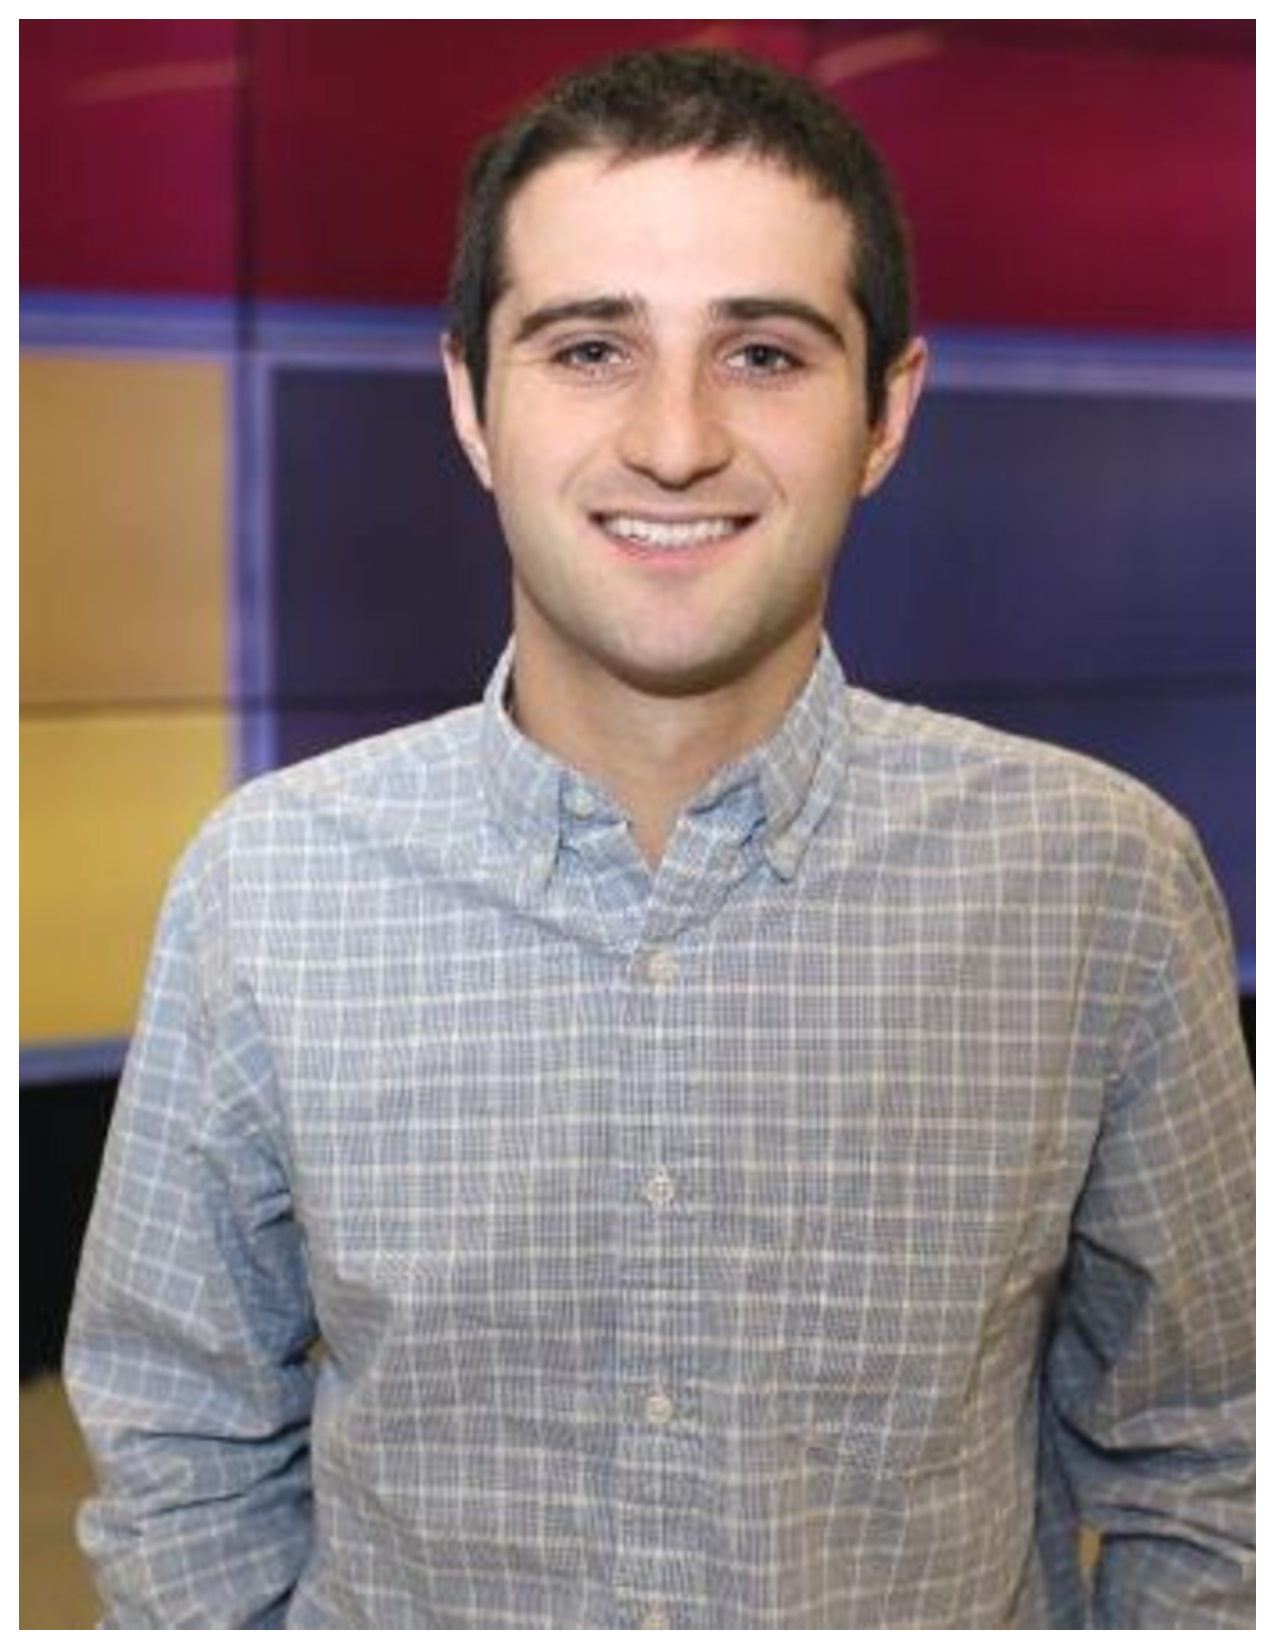
\includegraphics[width=0.25\columnwidth]{images/scott_mcclary}
  \end{wrapfigure}
  \noindent
  {\bfseries Scott McClary} received his BSc (Computer Science) and
  Minor (Mathematics) in May 2016 from Indiana University and will
  receive his MSc (Computer Science) in May 2017 from Indiana
  University. His research interests are within scientific application
  performance analysis on large-scale HPC systems. He will begin
  working as a Software Engineer with General Electric Digital in San
  Ramon, CA in July 2017.
\end{minipage}
\endgroup

\section*{} %used to create more spacing..
\section*{Work Breakdown}
The work on this project was distributed as follows between the
authors:
\begin{description}
\item[Scott McClary.] He completed all of the work for this project
  including researching, deploying, testing and benchmarking the CDMS
  application as well as composing this paper.
\end{description}

% Bibliography
\bibliography{references}
\end{document}

